\chapter{Comparing HAProxy and Pound load balancers}
\textbf{Keywords: Webservers, Performance, Analysis, Load Balancers, Scripting}

\subsection*{Abstract}
This chapter is a comparison of the two load balancers HAProxy and Pound, where
they are compared in the fields of Configurability, performance and
scalability. Through the testing of the different load balancers, a comparative
study will present the values of each load balancer.

\section{Introduction}
When thinking about the Internet today, most people associate this with the
Wold Wide Web. The reason for this is simple, as this is what everyday users use
daily. The main components to running the world wide web is the webservers,
which make all the content available through the HTTP and HTTPS protocols. 
These protocols have been around for a long while, where the first real
implementation were presented in 1992 with the first function of the GET
options \cite{w3:history}. The protocol were designed to transfer text files
over a \"telnet-style internet protocol\", but the protocol has evolved much
from the first iterations. \par

Last years there has been a shift in the way people use the Internet,
and with new streaming services like Spotify, Netflix and many other streaming
services, the webservers are getting more and more important. Other services
like social network, online banking, communications and almost anything
imaginable of information is mostly available. Although the information is out
there, this is not the only worry anymore. The information should be available
almost instant, and at the users demand. This is also included in one of the
most common security phrases; the CIA attributes: confidentiality,
integrity and \textbf{availability}.

All these services utilizes the power of the webservers, and the HTTP and HTTPS
protocols. But it is not possible to rely on one single machine to provide the
information to the masses. Not only because of general failure, but due to high
demand for the information, or the complexity of presenting it. A single server
can shutdown, but the information is still expected to be available.

To solve this problem, a layer between the end users and the webservers, called
a loadbalancer is introduced. This solution has the intention of spreading the
workload among the available servers and much more. These are the facility for
providing a more reliable World Wide Web, and to facilitate for high
availability and flexibility.

\subsubsection{Problem statement}

The given problem statement in this project was as follows:

\emph{Setup and evaluate and compare the HAproxy and pound load balancers for a
web- service with regard to:
\begin{itemize}
    \item Configureability
    \item Performance
    \item Scalability
\end{itemize}}

\section{Background}
Through this chapter we will focus on two different load balancers for load
balancing HTTP traffic. To be able to compare the load balancers, a short
introduction to the two different load balancers are needed, along with a
introduction to the concepts of balancing http traffic. How does a web server
work in short, and how is it possible to test the performance.

\subsection{Load balancing HTTP and HTTPS}
Load balancers are important to most of the high end websites that are
available. Ensuring high availability and scalability. They can be a part
of even the smallest sites that are prone to fail, ensuring high uptime,
or to balance the load over multiple web servers, or even database servers.

There are many different load balancers available. Many of these are open source
and free, but with varying quality and support. There are also many enterprise
load balancers or reverse proxy's as they are usually referenced to, like
Alteon product from Radware and Big IP from F5. But a load balancer could be as
simple as a single web server running apache or nginx.

The most basic feature of a load balancer is the ability to forward HTTP traffic
to the configured backends. The load balancer acts as a reverse proxy,
redirecting requests to one of the configured web servers. The algorithm used
for choosing server is normally some sort of least-connections or round-robin
distribution, distributing the load over the different web servers. The traffic
is then returned from the web server through the load balancer, to the client
that requested the specific page. Users do not see any of the actions of the
load balancer, making it a transparent service enabling high availability.

HTTP is the most common protocol for communicating with web servers, although it
does not provide any security measures. The security part is only implemented
in the HTTPS protocol, which implements security features like encryption and
web site verification with certificates. Some load balancers have the
possibility of terminating SSL connections. This would take the overhead of
encryption and decryption of traffic away from the web servers, and enable
the web servers to focus on the work needed to present the data.

SSL termination is just one of the many possibilities a load balancer for
HTTP/S brings to the table. It makes it possible to masquerade many servers
with different areas of expertise, like specific static content servers, and
dynamic content servers seem to be the same address, without the specific
handling in code. There are countless of possibilities, and load balancing is
now a must have for larger sites or site with the need for high availability.

%Backend,frontend, real server and vip is probably good to present

\subsection{HAProxy}
HAProxy is a powerful load balancer and reverse proxy. It has lots of
configuration possibilities, and large sites, like Reddit and Stackexchange 
use this tool to load balance their requests. \cite{haproxy:they_use_it}. 
It is a free software, that now comes packaged with the most common Linux 
distributions used, and is also supported by companies like Red Hat. 
HAProxy is written in C, and is therefore both lightwait and fast enabling
high performance load balancing. It can also be used to balance the TCP
protocol in general which means you can use it to proxy eg. databases. 

\subsection{Pound}
% why do we need to compare the balancers.
Pound is a open-source reverse proxy and HTTP load balancer designed to secure
applications. It is developed by Apsis, a security company, and created to
enable distribution of load over multiple web servers, and also to enable SSL
wrapping, for servers not offering this natively. It is a very small program
which is easily audited for security issues \cite{pound}.

% Talk about httperf
\subsection{Benchmarking with Httperf}
To benchmark both web servers and load balancers, a tool which can perform a
high number of connections to the web server at a short time interval is needed.
A tool like this is the Httperf tool created by HP. With this tool it is
possible to create a high number of HTTP or HTTPS requests to a website. This
is needed to see how the different component works under high pressure.
At one point there will be something that cannot handle the high load, but the
question is what the magical number would be. The key performance areas should
therefor be measured and evaluated, and this can be done with the output from
httperf.

The quality of the different performance benchmarking tools for HTTP, that are
openly available, are very variable. Httperf is a tool which does the job, but
it is old, and contain some bugs which you may find. Though httperf actually
can handle SSL connections, it does so only up to the standard of SSL 3.0. All
the versions of SSL/TLS up until version TLS 1.1 is broken with specific
ciphers (RC4). The performance testing of the handling of SSL/TLS is important, but
due to the differences in the SSL/TLS versions, and the unsupported usage of
httperf with these versions, this is not included in this comparison.

The best way to benchmark the different load balancers is therefor to test the
performance handling of HTTP with different loads. The easiest way to get
httperf is to install through the package manager in debian based systems. It
can also be compiled manually. This is needed to do testing with SSL/TLS, as
httperf needs the OpenSSL library. Httperf can be used to test the performance
with different connection rates, number of calls per connection and over a
longer period. An example of such a test is run with the following command:

\begin{lstlisting}[label=httperf, caption=Httperf output example,numbers=none]
httperf --hog --server balance2 --port 80 --uri /perf.php --num-conn 6000 --rate 100 --num-call 1 --timeout=5
httperf --hog --timeout=5 --client=0/1 --server=balance2 --port=80 --uri=/perf.php --rate=100 --send-buffer=4096 --recv-buffer=16384 --num-conns=6000 --num-calls=1
httperf: warning: open file limit > FD_SETSIZE; limiting max. # of open files to FD_SETSIZE
Maximum connect burst length: 1

Total: connections 6000 requests 6000 replies 6000 test-duration 59.995 s

Connection rate: 100.0 conn/s (10.0 ms/conn, <=3 concurrent connections)
Connection time [ms]: min 2.3 avg 3.1 max 60.5 median 2.5 stddev 1.1
Connection time [ms]: connect 0.5
Connection length [replies/conn]: 1.000

Request rate: 100.0 req/s (10.0 ms/req)
Request size [B]: 69.0

Reply rate [replies/s]: min 100.0 avg 100.0 max 100.0 stddev 0.0 (11 samples)
Reply time [ms]: response 2.6 transfer 0.0
Reply size [B]: header 167.0 content 8.0 footer 0.0 (total 175.0)
Reply status: 1xx=0 2xx=6000 3xx=0 4xx=0 5xx=0

CPU time [s]: user 30.92 system 28.78 (user 51.5% system 48.0% total 99.5%)
Net I/O: 23.8 KB/s (0.2*10^6 bps)

Errors: total 0 client-timo 0 socket-timo 0 connrefused 0 connreset 0
Errors: fd-unavail 0 addrunavail 0 ftab-full 0 other 0
\end{lstlisting}

The output of httperf gives information about the connection metrics, request
metrics, reply metrics, system metrics and errors during the test. This
information is important in finding the metrics of how the system is
performing. The command above can be explained as to run a test which lasts for
60 seconds, where total of 6000 connections are established, where 100
connections is established each second. It uses the \textit{--hog} option which
unlimits the usage of only 1024 ports for httperf to a range from 1024 to 5000.
Httperf uses this to use as many TCP ports as needed. The \textit{--server}
option specifies which server to connect to. The other options are important to
specify the number of connections and the time it will take for the test to
run. It is important to keep the rate of total connections and rate constant.

\section{Approach}
The operationalization asks for a study of two load balancers which can be
observed under the same conditions. There is therefor a need to have a
configuration and setup that is as similar as possible, so that the data
collected are comparative.

The two load balancers in question is th HAProxy and Pound load balancers. They
will be compared in regards to configurability, performance and scalability. 


% How thing is supposed to be set upk$
% Hypothesis

% assumption: set of assumption for the different cases
% should not be easy to find a saturation/cutoff point
% how the setup is
% The different cases:
    % httperf with increasing rate of requests and/or connections
        % naturally that there are multiple requests per connection
\subsection{Configurability}
% health check
% Documentation, configuration possibilities, ease of configuration file
The configurability of the two load balancers will be tested after the
installation and configuration. This will result in experience with the two
solutions and provide a view on how they are different. How the configuration
of the two solutions are will be based on the configuration options available,
with a special focus on the documentation provided. This especially since good
documentation is key to correct configuration of the system.

Through the documentation, the configuration possibilities are provided, giving a view on
the different possibilities the system gives to the user. There should be some
expected key points in the configuration where a given set of pre defined
options should be compared.

How the syntax of the configuration files is structured and viewable is
important to a system to ensure that misconfiguration does not happen. This is
a measure which is not directly quantifiable, but could be measured by counting
the number of characters used for specific operations. This should be used with
care, as more characters does not directly mean bad syntax. Through this the
usage of special characters could be used as a measure.

The configurability should also address the possibility of integrating outside
code into the load balancer, for either gathering metrics, or doing
configuration changes.

With this the following aspects needed to be addressed:
\begin{itemize}
    \item Configuration options
    \item Documentation and quality of documentation
    \item Syntax of configuration
    \item Integration possibilities
\end{itemize}

With the configuration options there is the need to set some specific
configurational attributes. The configuration options things that should be
present in the load balancers. 
\begin{itemize}
    \item HTTPS termination
    \item Management/Integration interface 
    \item Support
    \item Logging posibilities
    \item Graphical interface
    \item Documentation
    \item Requirements
    \item Balancing modes (algorithms)
    \item Cookie support
    \item IPv6
\end{itemize}

\subsection{Performance}
The benchmarking of load balancers is tricky. The expected result is not to
actually find the saturation point. HAProxy as an example has been reported to
successfully handle the load of a full 1 gigabit ethernet connection, and does also
handle the loads of large pages \cite{haproxy:2014}. To test the performance of
the different load balancers, the key aspects should be the usage of system
resources. High amount of forking or many system calls can actually
lead to slower performance of the system, and cause the hardware or platform to
be more powerful. This is a key aspect to the performance. It is not expected
to find the breaking point, but with this it is possible to find the surrogate
values that could provide an answer to if the application could fail in the
feature and with higher load.

While doing the performance testing, a webpage is needed on each of the
backends. Since it is the load balancer that is tested, it is important that
the backend servers will not get saturated through high load. This can be done
by using a php script which uses the sleep function. This ensures that the web
requests take longer time, but still does not cause high CPU iterations on the
backends. Some tests of different web pages shows that a normal response time
is about 0.2 seconds. This is also around the time for cognitive response to be
observed, and if a request take longer than this time limit, the user would
observe the page as loading. The value of 0.2 seconds is therefor chosen, and
the two load balancers should be tested with this sleep time. The response time
relative to this should be tested, so that the basic user experience can be
shown.

To test the performance of the load balancers, httperf will be used. To be able
to collect the information gathered from httperf, a script that can parse the
output of the tool is needed.

\subsection{Scalability}
There are different parts of the object of scalability. The load balancer
should be able to handle many backend servers, but should also handle the
possibility of failover from the running instance, enabling multiple load
balancers to run. Having only one load balancer running, would result in a
single point of failure.

One site may have one or more load balancers, but there are usually a lot more
applications than just the single web applications that are expected here. It
should therefor be possible to create multiple frontends in the load balancer
along with multiple backends, and map these respectively.

The quantitatively measure of this, could possibly be found in the
documentation of the load balancers if the documentation is good. This will
provide a input on how many frontends, backends and possible backend servers
that are configurable.


\section{Result}
%What happened
% os limits
% sudo apt-get install autoconf libtool -y
% https://rtcamp.com/tutorials/benchmark/httperf/
% before make install run ulimit -n 65535

% Subsection: Configurability
%   Syntax? Functions, documentation, community and continuous support (new
%   versions?) This is relevant, but not directly to how it works. Evaluate
%   this!
%
\subsection{Configurability}
Through the points set in the approach the different points of the two load
balancers can be viewed.

\subsubsection{HAProxy}
HAProxy is a well formed load balancer, which is beautifully implemented. The
documentation on the website \ref{haproxy:configuration_manual} is well
written, and complete with performance tuning options and a lot of
information. The documentation is split into different parts; Configuring
HAProxy, Gloabl parameters, Proxies, Bind and Server options, HTTP header
manipulation, Using ACLs and fetching samples, Logging and Statistics and
monitoring is the main parts. A lot of performance tuning options are available
where an advanced options can be tuned to get the best performance for your
system. The tests that has been done in this report does not take advantage of
any of these.

The configuration file is split neatly into three main parts. The
\textit{global}, \textit{frontend} and \textit{backend}. The global part
contains all the global configuration \vref{lst:haproxy.cfg}. The frontend part
is extendible, and for each application, a new frontend should be added. For
the backends it is the same, as a backend represents a list of available servers
for a frontend.

The syntax of the configuration is nice, where indentation is used. There is
not a lot of special characters, making the configuration file easy to read.

Integration is also possible through the socket connection available. This
requires an application running on the same server, as this is a local socket,
and not a network socket. Through this socket connection, there is options to
set the server in maintenance mode, and other modes runtime. There is no option
for adding servers through the socket connection. This is OK, as it will
maintain a complete configuration file, and ensuring that every configuration
option is stored in the configuration file.

\subsubsection{Pound}
Pound is a more lightweight load balancer compared to HAProxy, and has less
records of success posted on their web page.
The documentation of pound is sparse \cite{pound}. Although it has a well
formed man page, with configuration examples and some descriptions of the
different options.

Though there is performance tuning options in the configuration documentation,
it seems like the most important function for a small scale site is present,
making it possible to create a high available site.

The configuration file of pound, \vref{lst:pound.cfg}, is compared to HAProxy
messy. It Uses many of the same features, but have some other naming
convention. It also practices start / end blocks of each option, shown in the
minimal configuration. There is no excessive usage of special characters which
is good, but it uses on the other hand keywords in camel casing, which makes
the configuration file look more messy. It gets bad when adding many different
backends, as each backend is followed by a block with the naming \textit{END}.

For runtime configuration, there is a tool called poundctl which enable
connection to the socket presented. This gives the same functions as available
with the socket interface natively. This includes enable/disable a listener,
service or backend. The tool is old, but still works.

\subsubsection{Comparison of features}
A short comparison of the different features found in HAProxy and Pound.
\begin{table}[h]
\begin{tabular}{lll}
\hline
Feature                 & HAProxy                                       & Pound                       \\ \hline
HTTPS termination       & Yes                                           & Yes                         \\ \hline
Socket connection       & Yes                                           & Yes                         \\ \hline
Logging possibilities   & Configurable to capture traffic and much more & Syslog or stdout            \\ \hline
Graphical interface     & Web statistics overview                       & None                        \\ \hline
Documentation           & Really good documentation                     & Sparese                     \\ \hline
Requirements            & OpenSSL for SSL termination                   & OpenSSL for SSL termination \\ \hline
Balancing modes         & 10 different. Incl. most common               & Unknown                     \\ \hline
Session/ Cookie support & Yes                                           & Yes                         \\ \hline
IPv6                    & Yes - IPv6 to IPv4 support                    & Yes - IPv6 to IPv4 support  \\ \hline
\end{tabular}
\end{table}


\subsection{Performance}
To be able to do the tests needed to run httperf with an incremental mode, and
getting the data from httperf, a opensource project on Github has been used.
This project called Httperfpy \cite{httperfpy} can based on the input given to the class
constructor, run httperf with the options given, and if specified parse the
output. Httperpy did have some things missing, like the possibility of passing
\textit{--hog} to httperf. The changes necessary for adding this option were
added, and submittet back to the project based on the following pull request
\cite{httperfpy:pull_req}, which is added and now available in the pypi
package.

The script used for running the performance tests is added as appendix
\vref{lst:run.py}. The script takes the output of httperf and parses it, before
it appends it to a csv file for the current measurement. This makes the project
repeatable, and there is not a lot of prerequisites needed to perform the tests.
The csv file created will have the following format, where the new measurements are appended to the
file:

\lstinputlisting[label=lst:perf_data,caption=Data output of a combined
run, numbers=none, firstline=0, lastline=2]{chapter2/data/data_show}

% each test is run three times
The following graph is a plotting of the response times gotten from the csv
file above.
\begin{figure}[H]
\centering
\makebox[\textwidth][c]{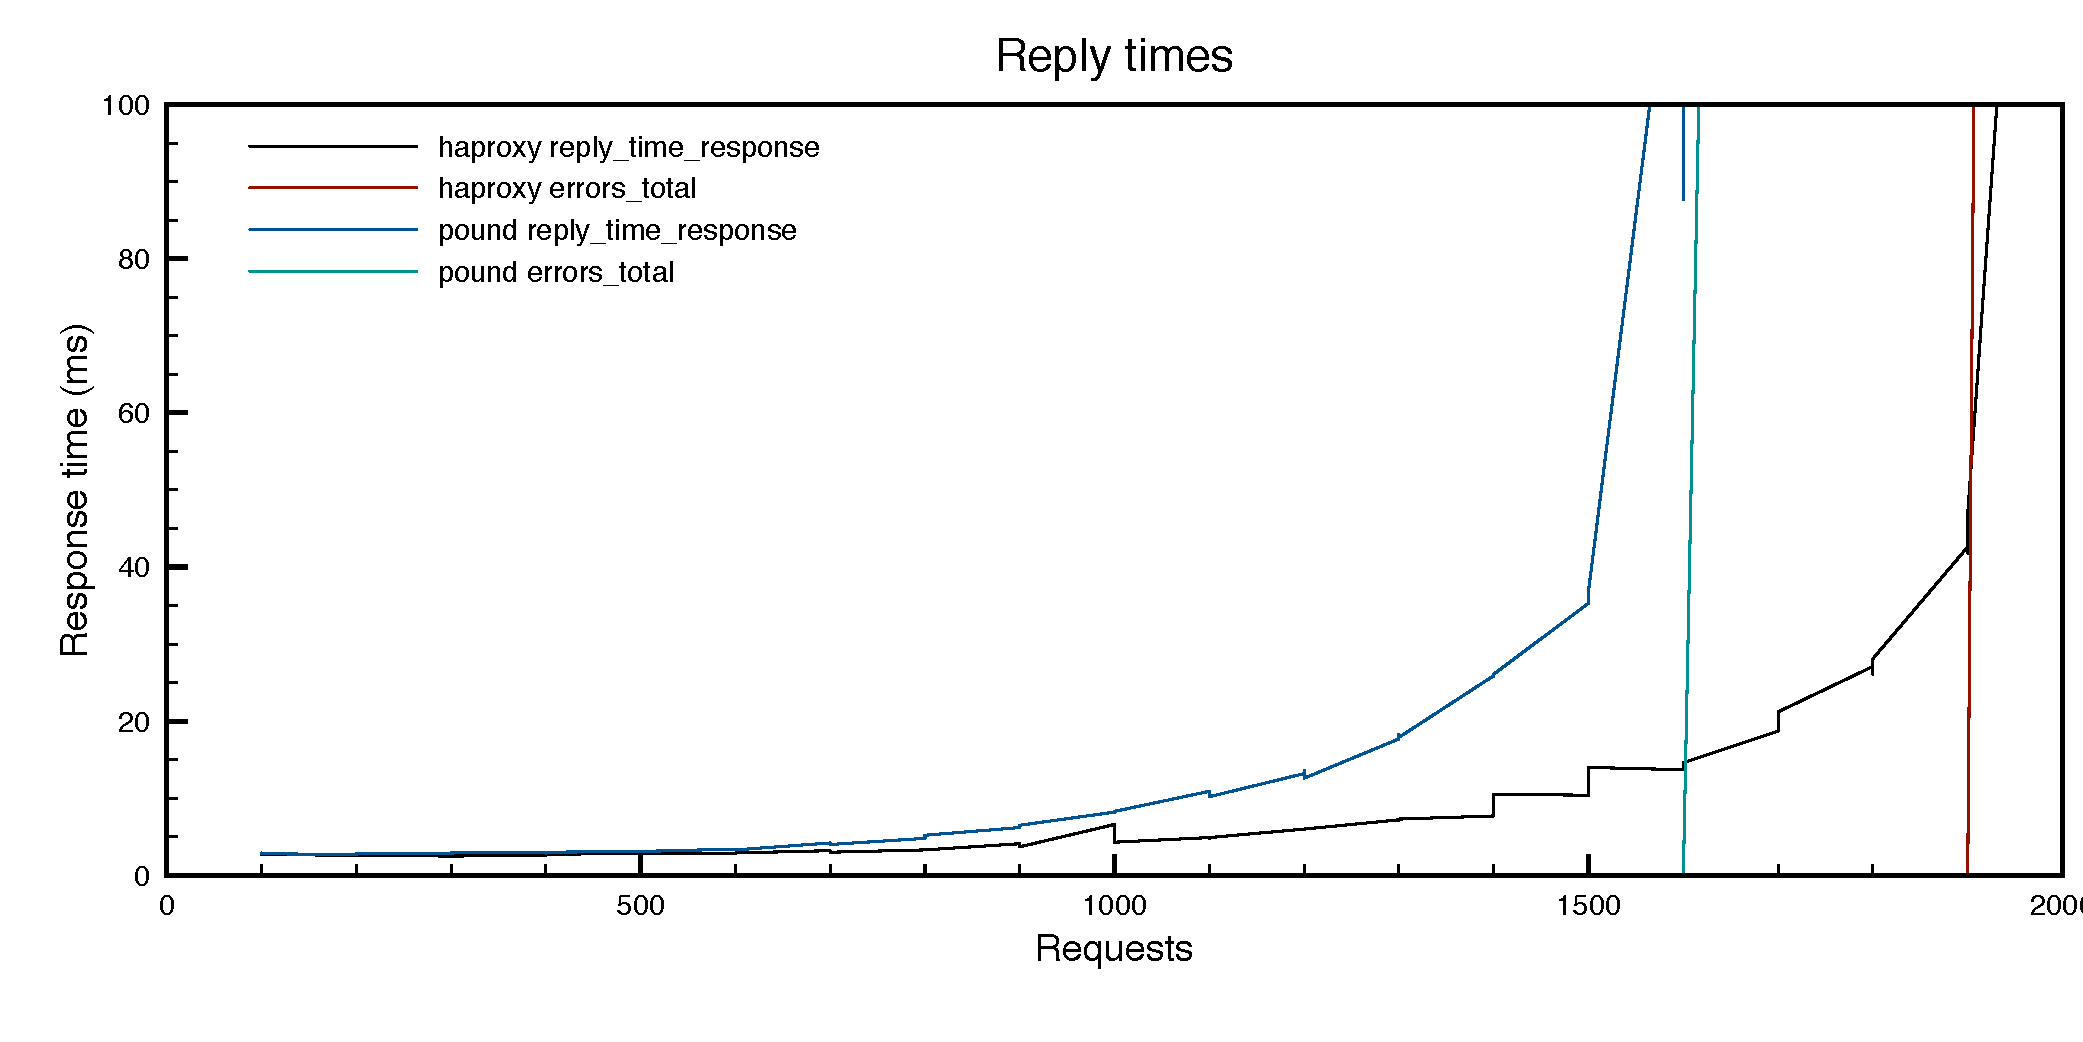
\includegraphics[width=1.25\textwidth]{chapter2/reply_times}}
\caption{\label{fig:reply_times}Reply times from the two load balancers}
\end{figure}

At the same time as the tests have been running, the CPU usage have been
monitored on the load balancers. From the following graph the CPU utilization
is visible. The test that has been running with this graph is an incremental
test from 100 until 2000 requests a second at a incremental value of 100
requests. Each test were run 3 times. To measure these values, the \textit{sar}
command has been used to capture the CPU usage.
This has simply been done by using the following command, which captures the
CPU usage every second second.
\begin{Verbatim}[frame=none]
$ sar -u 2 4000 >> cpu_mon_balance*
\end{Verbatim}

\begin{figure}[H]
\centering
\makebox[\textwidth][c]{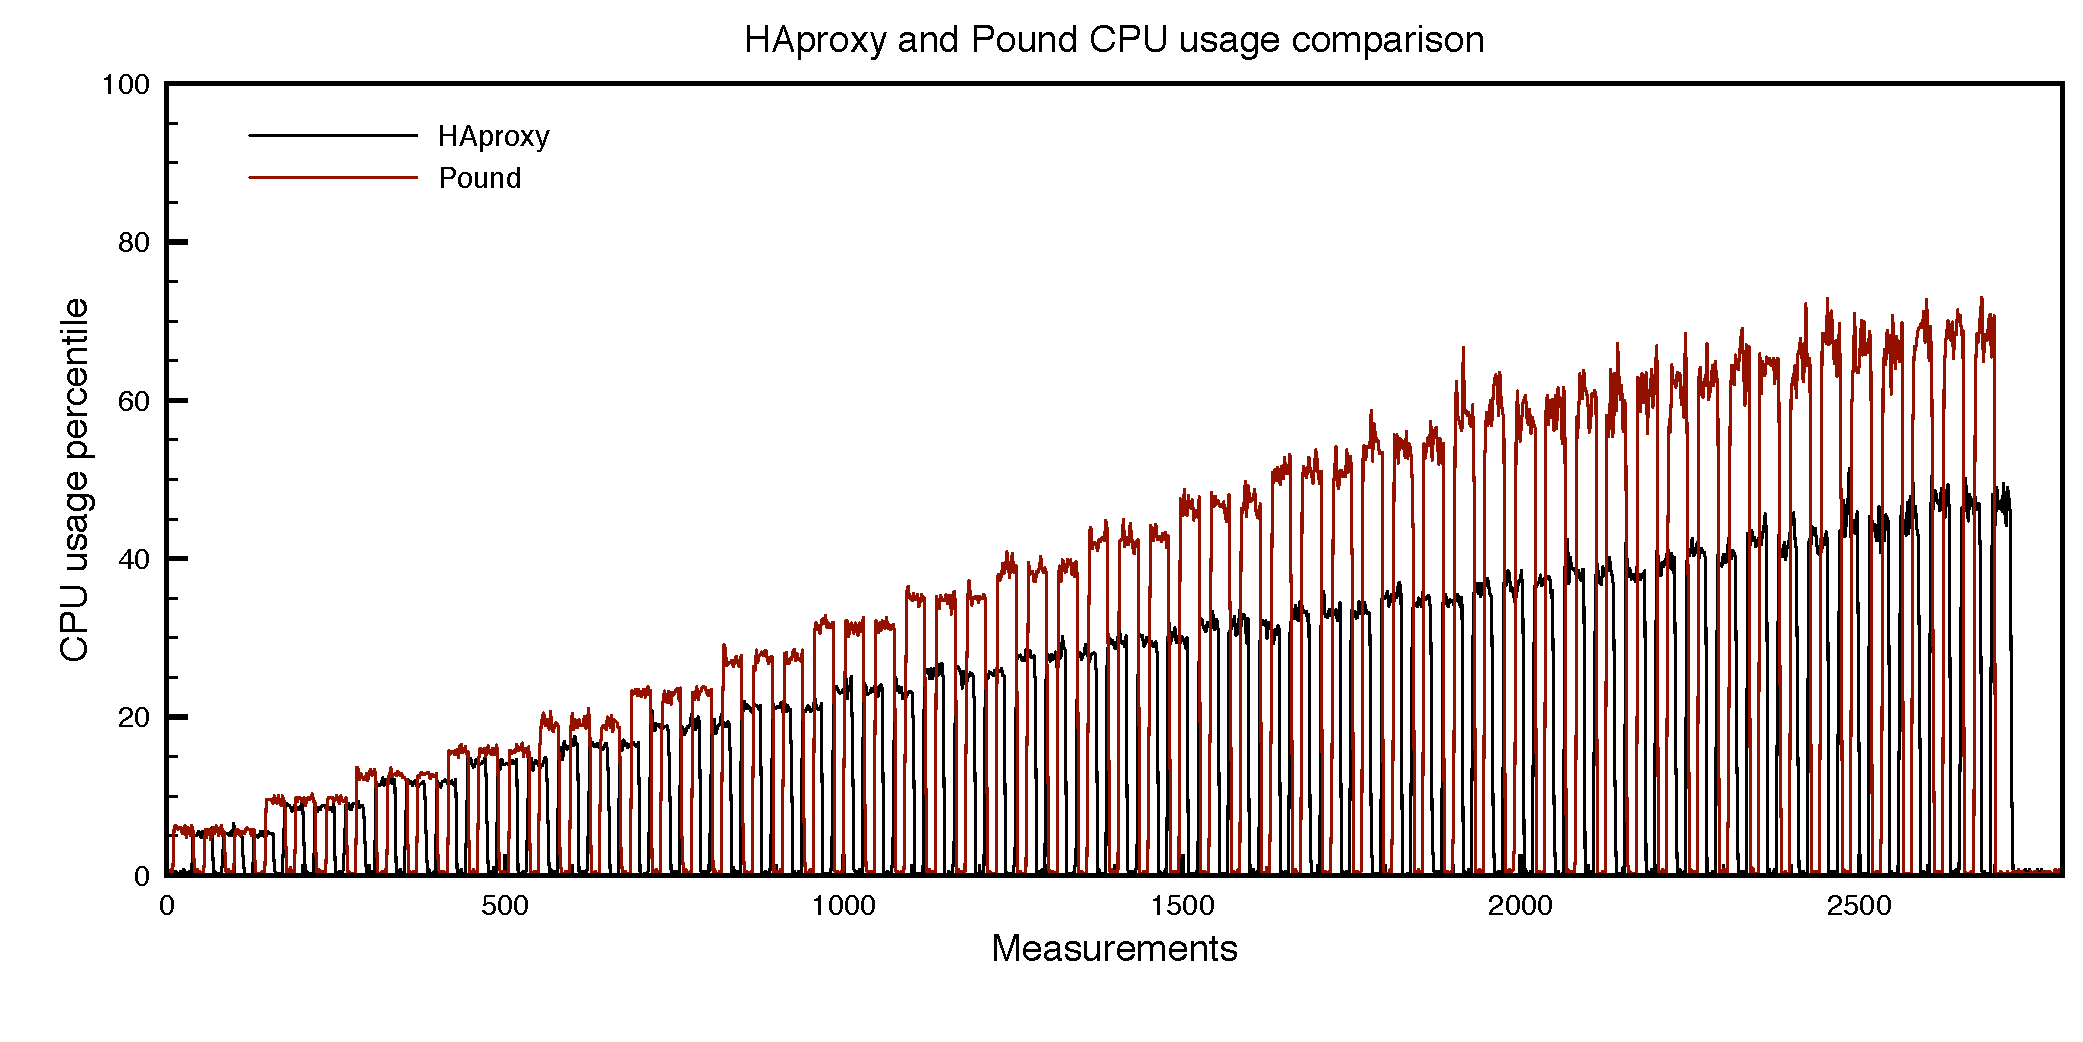
\includegraphics[width=1.25\textwidth]{chapter2/cpu_usage}}
\caption{\label{fig:cpu_usage}Cpu usage of HAProxy and Pound under different
loads}
\end{figure}

\subsection{Scalability}
There are many possibilities with both Pound and HAProxy. HAProxy is probably
the most mature of the two, where it is possible to synchronize the connection
table of HAProxy to another HAProxy instance. With the usage of keepalived, it
is possible to create a high availability setup with HAProxy. This is
documented well by Red Hat \cite{redhat:haproxy}.
This is not very well documented in regards to Pound, so if this is possible,
it is a good kept secret.

How many frontends and backends it is possible to add or use, and the
performance impact of said configuration is something that is not covered well
here. The documentation of either does not state the limitations on this
aspect, which leads to assume that there is a lot more than what is necessary
for normal usage.

% the data are presented as described in the approach section
% how are the tests run
% sample output of scripts and/or httperf
% present the data for the spesifik sets
    % how to find the data and how they were analyzed


% ssl signing: openssl req -x509 -sha256 -nodes -days 365 -newkey rsa:4096
% -keyout mycert.pem -out mycert.pem

\section{Analysis}
 %Look at the data
 % Analyze the hypothesis
 The data gathered in the results, presents to important graphs. We can from
 \vref{fig:reply_times} see that there is a difference in the way that HAProxy
 and Pound manages to respond to the requests. Already at 1000 requests per
 second, there is a noticeable difference, ant at 1500 requests per second
 Pound does not follow at all. The reason for this could be that the fd limit
 is set on the balancer, and this is also shown when the errors come. These
 errors are fd limit errors, and is not a key value for saying anything about
 how the balancer is handling. 

 With the information gathered about system resources we can see that there is
 a significant difference in the way that HAProxy and Pound work. Shown in
 \vref{fig:cpu_usage} it shows that Pound uses as much as 20\% more CPU than
 what HAProxy does.
 A reason for this could be that Pound forks new threads for each new
 connection, and has therefore a lot of system calls for each connection,
 whereas HAProxy is a single threaded process of effective code that has to do
 a lot less system calls than what of Pound.

\section{Discussion and conclusion}
A lot of data has been captured to be able to gather some information about the
load balancers. This has mostly been gathered from httperf, but also system
values with tools like sar. There is a lot of data that is captured, and more
of this data could be graphed, as they make little meaning by themselves. This
is one of the improvements that is needed to further sturdy the comparison of
these load balancers.

It is important to note that the data gathered from the usage of httperf is
done with the package manager of httperf with the fd\_limit set. This can be a
problem, and the errors has therefor been plottet in the graphs. The load
balancers are also configured with the fd\_limit set, meaning that both
balancers will notice these errors, but will handle them differently.

 It is not possible to be sure about any saturation point for both balancers,
 as the data gathered most likely show some sort of external effect from the
 operating system. This means that if the operating system and the load
 balancers were perfectly configured, a more accurately test could be done.


\subsection{Improvements}
% SSL and why we dont care here. 
% Other possible benchmarking tools?
% large files transfer rate
% system is not configured for high load

There is a lot of improvements that could be done to this task, and there is
still a lot of work to be done to be 100\% sure of the results that are
gathered. Some of the main improvements are the usage of SSL to test one of the
most important features of these load balancers. The test does also only test
the connection rate, and does not look at how the load balancers behave when
higher sizes are forwarded. This would be relevant to video streaming and the
like. The system should be configured for higher load to be able to accuracy
measure the performance of the load balancers, as the setup today does not
provide a perfect solution. 

There are many other improvements that could be done to this testing, and
although this gives a picture on the two load balancers, it is not a complete
picture.

\subsection{Conclusion}
In summary, the task has been completed to some degree. There is still a lot of
work left to have a complete finished performance comparison, and evaluation of
the two laod balancers, but it is possible to get some key points from the
information gathered. 
It is possible to conclude that HAProxy seems to be the best tool for the job
in both smaller scale, and larger scale when it comes to configurability, both
due to the amount of configuration possible, the good documentation and the
beautiful configuration file.

Performance wise, HAProxy also has a small leap in front of Pound, where it has
better response times at higher load, and also uses a lot less processor power. 

Scalability is a topic that is not widely touch on here, but it is possible to
see that HAProxy has an advantage in the possibilities of using keepalived.

\section{Appendix}
\begin{center}
\lstinputlisting[label=lst:run.py, caption=Script for running httperf through
httperfpy, language=Python]{chapter2/run.py}

\lstinputlisting[label=lst:perf.php, caption=Webpage used for benchmarking,
language=php]{chapter2/perf.php}

\lstinputlisting[label=lst:haproxy.cfg, caption=HAProxy configuration
file]{chapter2/haproxy.cfg}

\lstinputlisting[label=lst:pound.cfg, caption=Pound configuration
file]{chapter2/pound.cfg}

\lstinputlisting[label=lst:plot2_import, caption=Script for getting csv data into
plot]{chapter2/plot2_import.pl}
\end{center}
